%compile with pdflatex on papeeria

\documentclass[a4paper,12pt]{article}
\usepackage{fancyhdr}
%\usepackage{fancyheadings}
\usepackage[ngerman,german]{babel}
\usepackage{german}
\usepackage[utf8]{inputenc}
%\usepackage[latin1]{inputenc}
\usepackage[active]{srcltx}
%\usepackage{algorithm}
%\usepackage[noend]{algorithmic}
\usepackage{amsmath}
\usepackage{amssymb}
\usepackage{amsthm}
\usepackage{bbm}
\usepackage{enumerate}
\usepackage{graphicx}
\usepackage{ifthen}
\usepackage{listings}
\usepackage{enumitem}
%\usepackage{struktex}
\usepackage{hyperref}
\usepackage{tikz}
\usepackage{float}
\usepackage{subcaption}
\captionsetup{compatibility=false}
\captionsetup[subfigure]{labelformat=empty}

\usepackage{pgfplots}
\usepgfplotslibrary{fillbetween}
%\usetikzlibrary{patterns}
\pgfplotsset{compat=1.15}
\usepackage{mathrsfs}
\usetikzlibrary{arrows}

\pgfplotsset{grid style={dashed,gray}}

\definecolor{kolorwykresu}{rgb}{0.07,0.04,0.56}

\pagenumbering{gobble}

%% Aufgaben-COMMAND
\newcommand{\Aufgabe}[1]{
  {
  \vspace*{0.5cm}
  \textsf{\textbf{Aufgabe #1}}
  \vspace*{0.2cm}
  
  }
}
%%%%%%%%%%%%%%
\lstset{ %
language=java,
basicstyle=\footnotesize\tt,
showtabs=false,
tabsize=2,
captionpos=b,
breaklines=true,
extendedchars=true,
showstringspaces=false,
flexiblecolumns=true,
}

\begin{document}


{\bf ANALYSIS}\\

%\hline
Betrachtet werden Funktionen vom Typ $f(x) = \frac{a(x+b)(x-c)}{x^n}$ mit natürlichen Zahlen $a, b, c, n$. ($n\ge2$)


\begin{enumerate}[label={\alph*)}]
  \item Bestimmen Sie die Nullstelle(n) und die maximale Definitionsmenge.
  \item Ermitteln Sie die Gleichungen aller Asymptoten.
  \item Die folgende Abbildung zeigt den Graphen einer solchen Funktion

\begin{figure}[ht!]
\centering
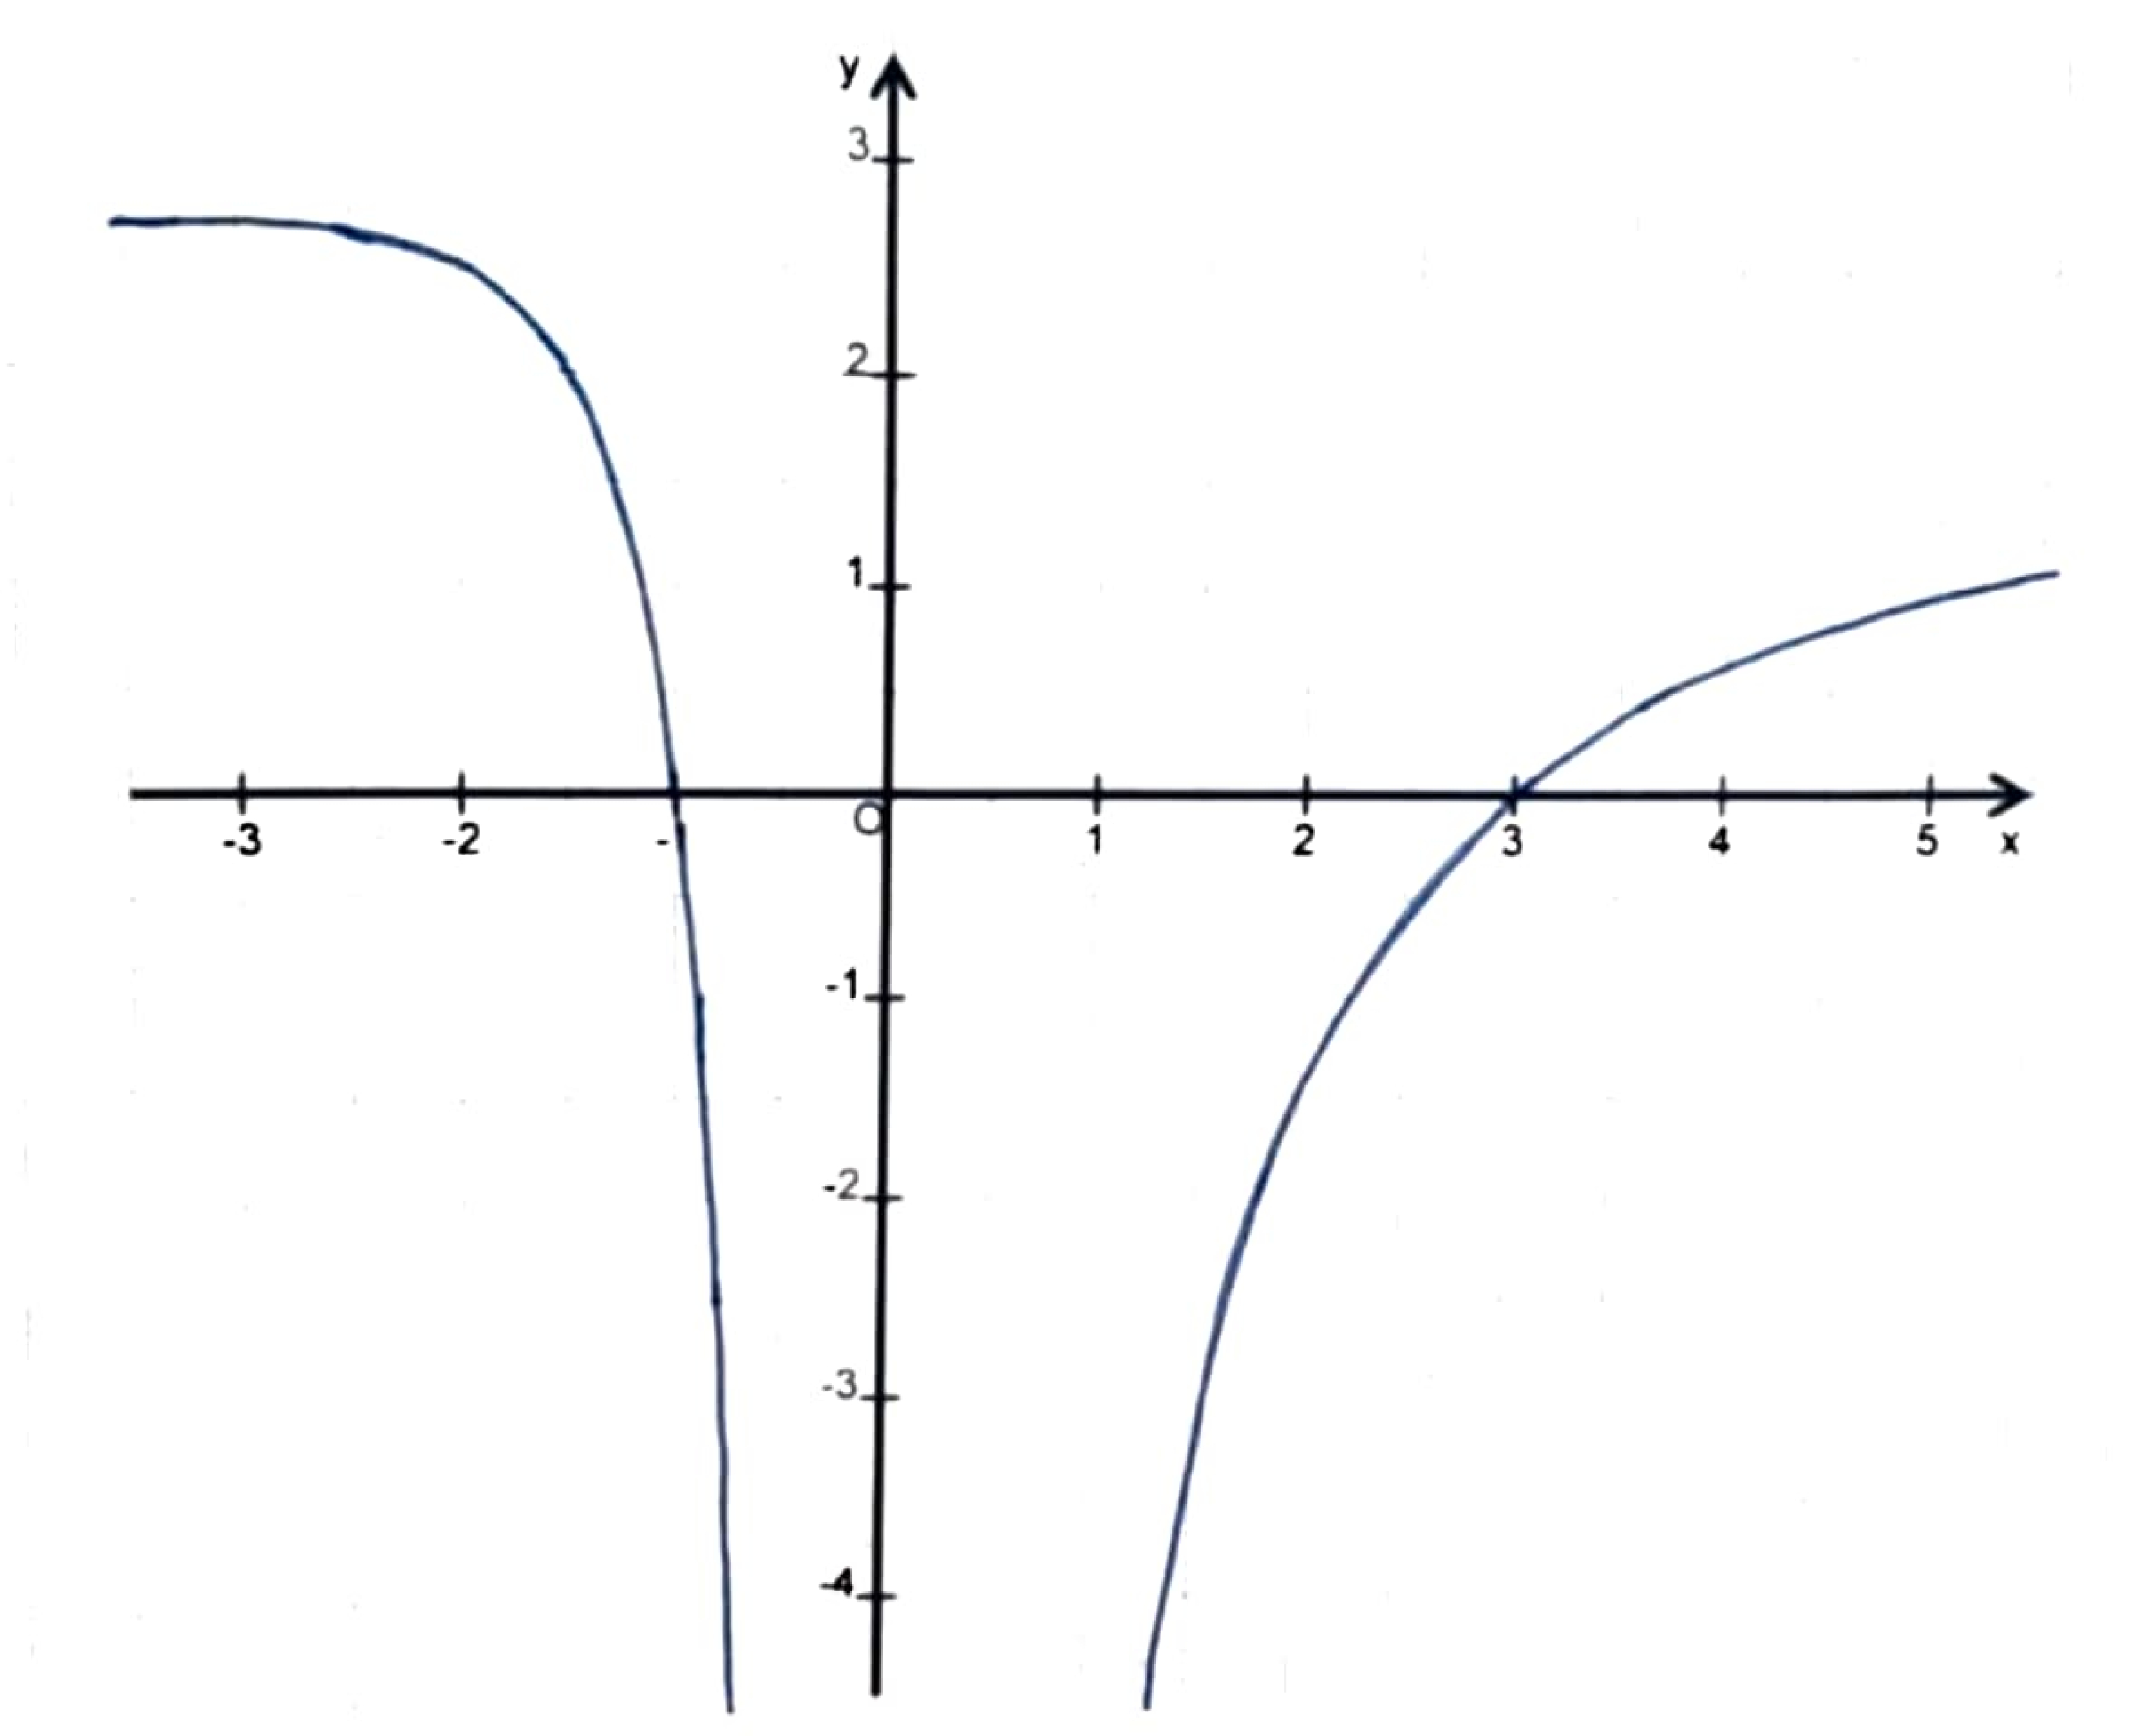
\includegraphics[width=90mm]{g1.jpg}
\end{figure}

Geben Sie einen möglichen Satz von Parameterwerten an und begründen Sie Ihre Wahl.
\end{enumerate}

{\bf Vertiefungsfragen}\\

Zeichnen Sie in die Abbildung die Graphen der folgenden Funktionen ein: 
\[ g:x \rightarrow g(x) = f'(x); D_g = D_f\]
\[ l:x \rightarrow l(x) = \int^{x}_{2}f(t)dt; D_l = {\mathbb{R}}^{+}\]


\newpage

{\bf GEOMETRIE}\\
In einem kartesischen Koordinatensystem sind die Punkte $A(2|6|0)$, $B(1|-2|5)$ und $C(-1|6|3)$ gegeben.

\begin{enumerate}[label={\alph*)}]
  \item Bestimmen Sie einen Punkt $P$, der im Inneren des Dreiecks $ABC$ liegt, d.h. auf der Dreiecks fläche, aber nicht auf dem Rand.

 \item Beschreiben Sie einen möglichen Weg zur Überprüfung, ob das Dreieck $ABC$ rechtwinklig ist\\ 
   {\bf Vertiefungsfrage:} Reicht es aus, wenn man zwei Skalarprodukte ungleich Null berechnet hat?

  \item Geben Sie an, auf welche Weise die Gleichung der Ebene $E$ in Normalenform aufgestellt werden kann, die das Dreieck $ABC$ enthält. (Mögliches Ergebnis: $2x_1 + x_2 + 2x_3 -10 = 0$).

  \item Bestimmen Sie einen Punkt $P$, der den Abstand $10$ zur Ebene $E$ hat.

  \item Gegeben ist zusätzlich die Gerade $g: \vec{X}=\begin{pmatrix} -1 \\ 6 \\ 3 \end{pmatrix} + \lambda \cdot \begin{pmatrix} 4 \\ 2 \\ 4 \end{pmatrix}$

  Beschreiben Sie die Lagebeziehung zwischen g und dem Dreieck $ABC$.
\end{enumerate}


{\bf Vertiefungsfrage}\\
Das Dreieck $ABC$ lässt sich durch Hinzunahme eines weiteren Punkts zu einem Parallelogramm ergänzen. Erklären Sie an einer Skizze, wie viele verschiedene Punkte hierfür infrage kommen, und erläutern Sie für \textit{einen} davon, wie man seine Koordinaten ermittelt.\\

{\bf ZUSATZFRAGEN}\\

\underline{Geometrie:}\\

Für drei Punkte $U, V, W$ gilt $\overrightarrow{UV} \times \overrightarrow{UW} = \vec{0}$ und $ \overrightarrow{UV} \circ \overrightarrow{UW} < 0$.\\
Skizzieren Sie eine mögliche Anordnung der drei Punkte.\\

\underline{Analysis:}\\

Zu einer gegebenen Funktion $f$ gibt es i.d.R. mehrere Stammfunktionen und mehrere Integral funktionen. Zeigen Sie an einem selbstgewählten, konkreten Beispiel, dass nicht jede Stamm funktion zugleich eine Integralfunktion ist.\\

\newpage


{\bf ANALYSIS}\\

\begin{enumerate}
  \item Die Abbildung zeigt den Graphen $G_k$, der Ableitungsfunktion $k'$ einer Funktion $k$. Die beiden Nullstellen von $k'$ werden mit $x_1$ und $x_2$ bezeichnet, wobei $x_1 < x_2$ ist.

\begin{figure}[ht!]
\centering
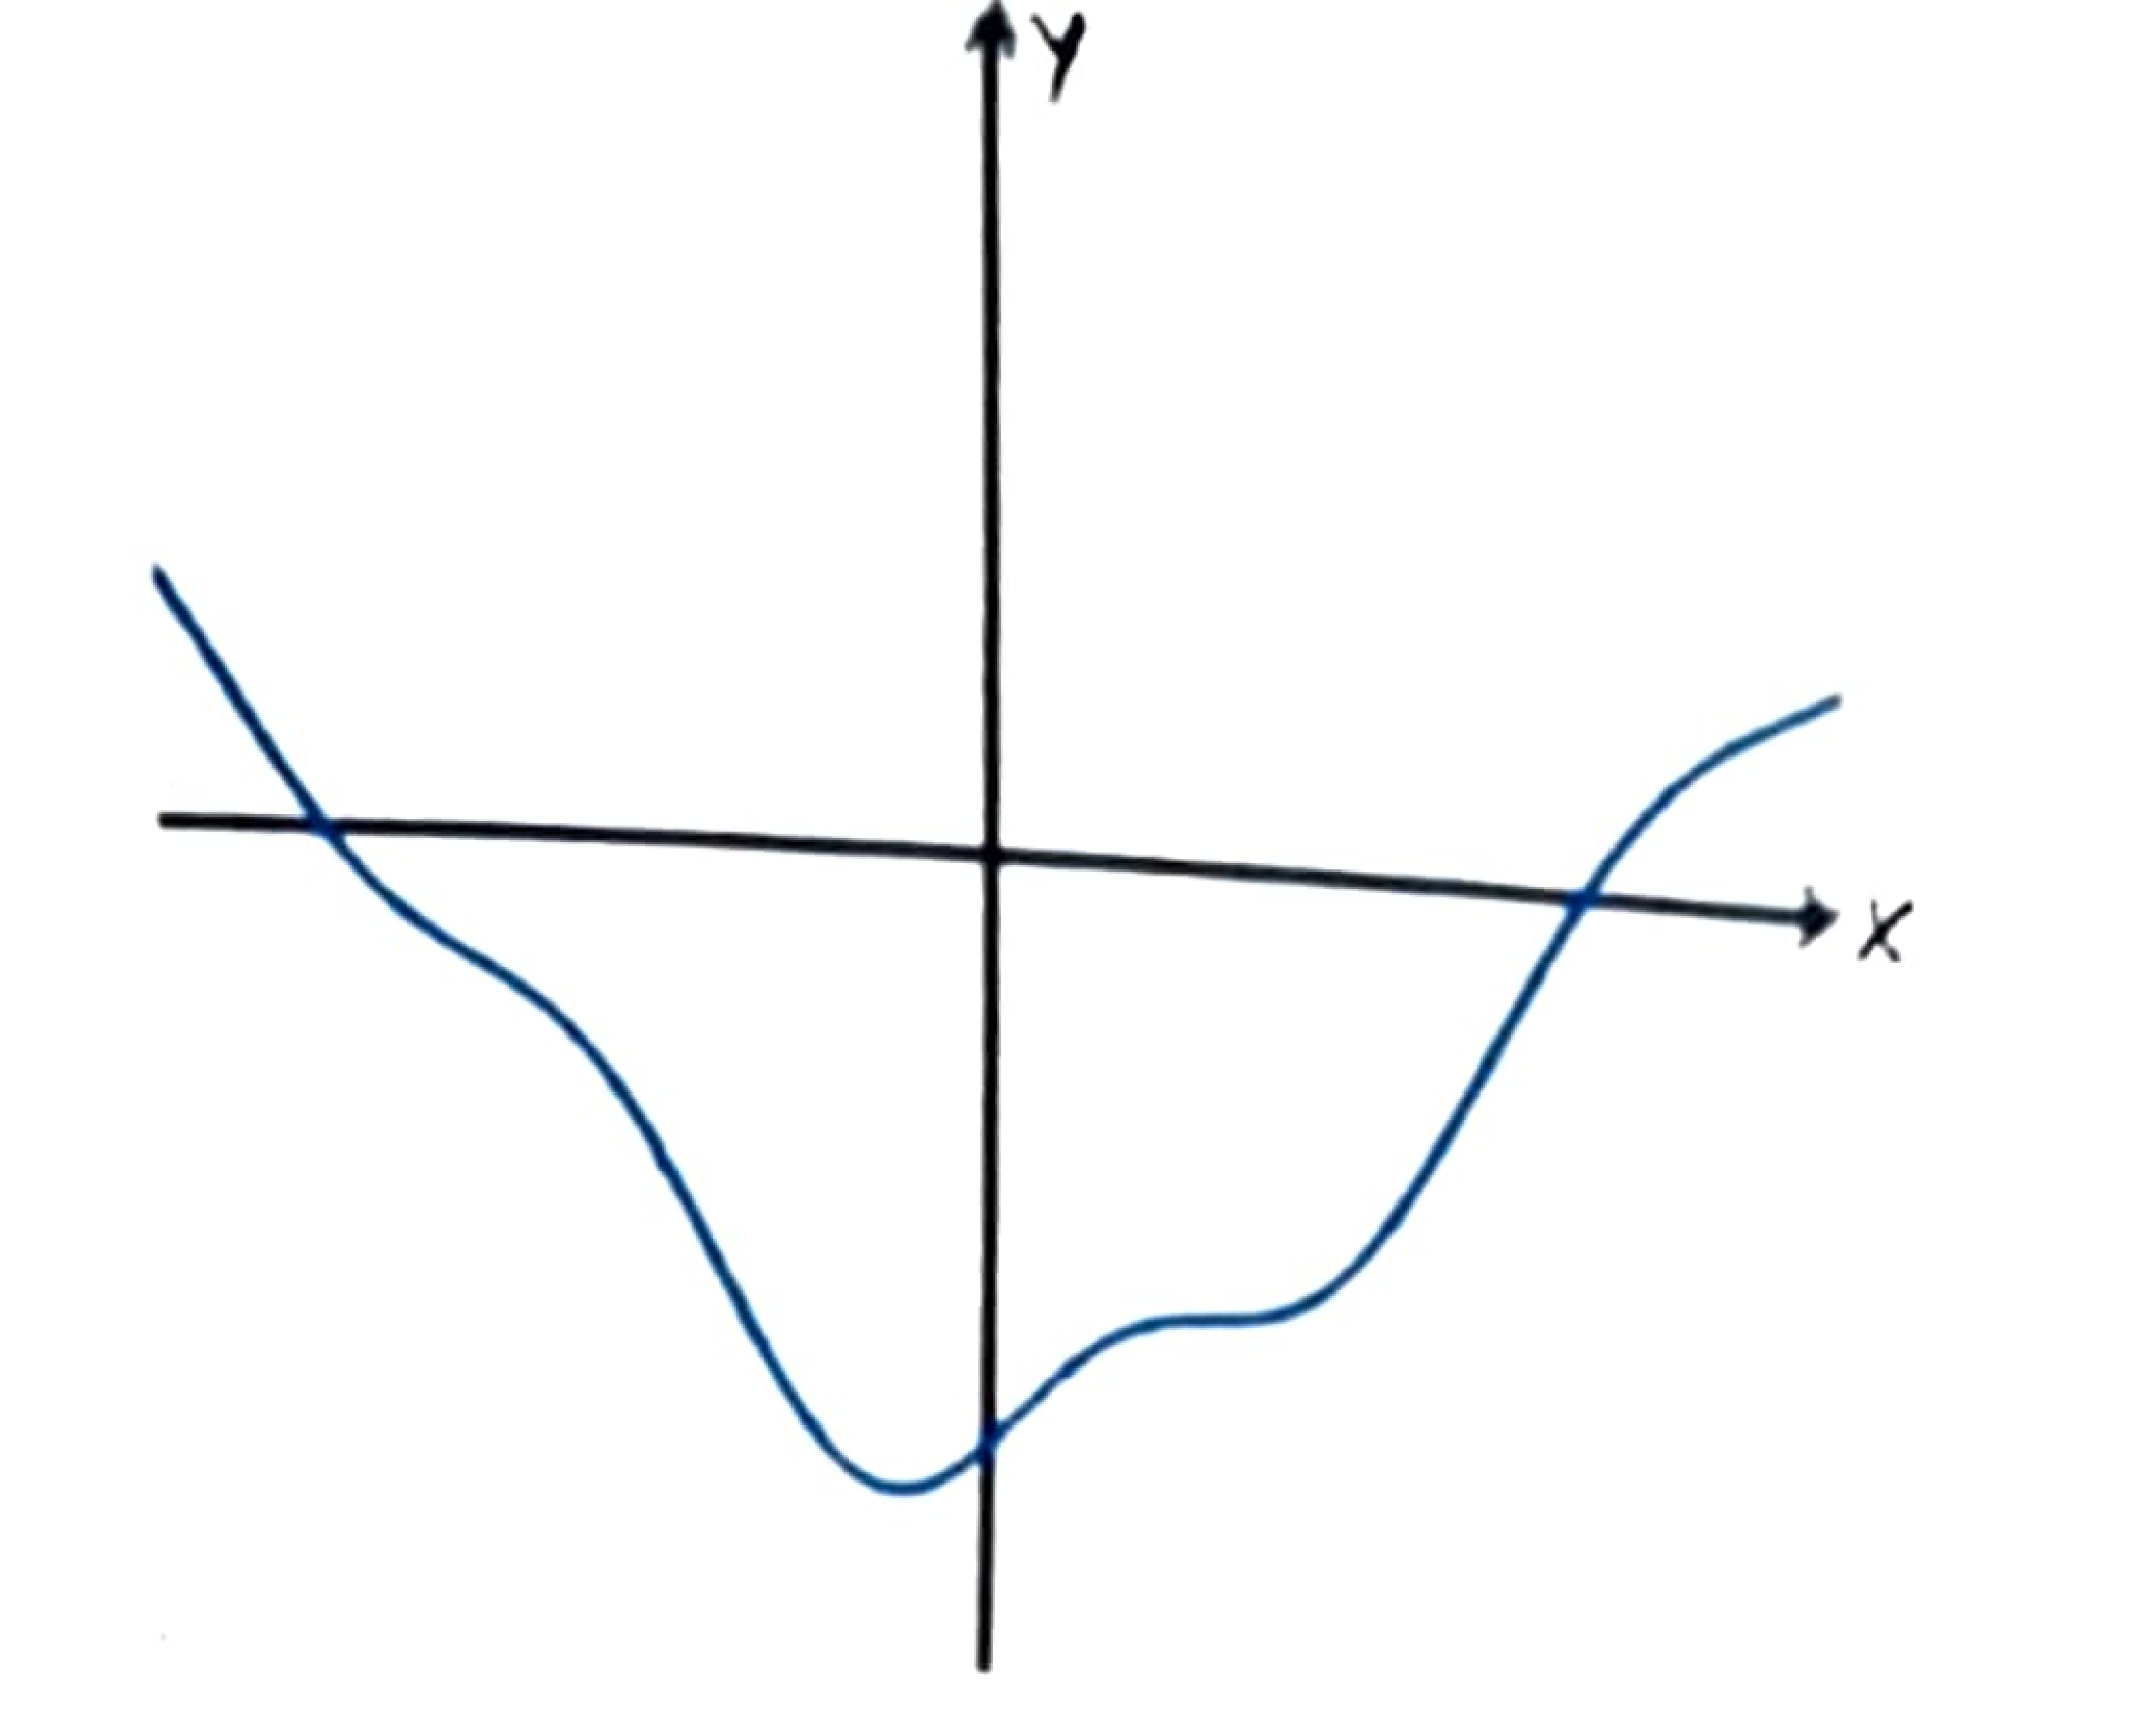
\includegraphics[width=50mm]{g2.jpg}
\end{figure}


      \begin{enumerate}[label={\alph*)}]
        \item Geben Sie zu jedem der folgenden Ausdrücke an, ob damit der Inhalt des von $G_k$ und der $x-$Achse eingeschlossenen Flächenstücks korrekt wiedergeben wird.\\

      \begin{tabular*}{\textwidth}{c @{\extracolsep{\fill}} cc}
        $\int_{x_1}^{x_2}|k'(x)| dx$ &
        $|\int_{x_1}^{x_2}k'(x) dx | $ &
        $k(x_1)-k(x_2)$ \\
      \end{tabular*}\\

      \item Das Flächenstück aus Teilaufgabe a habe den Inhalt 64 [FE]. \\
            Bestimmen Sie, davon ausgehend, Näherungswerte für $x_1$ und $x_2$.
    \end{enumerate}

  \item Gegeben sind zwei Funktionen $G$ und $H$ mit $G(x)=\frac{x}{x-0,5}$ und $H(x) = (2x-1)^{-1}$ ihrem jeweiligen maximalem Definitionsbereich.

      \begin{enumerate}[label={\alph*)}]
        \item Zeigen Sie, dass folgende Aussagen zutreffen:
          \begin{enumerate}[label={(\arabic*)}]
            \item Genau eine der beiden Funktionen besitzt eine Nullstelle. 
            \item Die Graphen beider Funktionen besitzen genau zwei Asymptoten.
            \item $G$ und $H$ sind zwei verschiedene Stammfunktionen der gleichen Funktion $f$.
          \end{enumerate}

          Im Folgenden dürfen die obigen Aussagen als bewiesen vorausgesetzt werden.

        \item Begründen Sie, ob sich $G$ bzw. $H$ als Integralfunktion in der Form $l(x) = \int_{a}^{x} f(t) dt$ schreiben lässt.
      \end{enumerate}
    \end{enumerate}


\textbf{Vertiefungsfragen:}\\
zu 2) Erklären Sie anschaulich, was sich aus Teilaufgabe 2a über die gegenseitige Lage der Graphen von $G$ und $H$ folgern lässt.\\
zu 1) Erklären Sie mithilfe des abgebildeten Graphen ausführlich, wo der Graph von $k$ eine Wendestelle besitzt.


\newpage


\underline{\textbf{STOCHASTIK}}\\
\begin{enumerate}
  \item In einer Verkaufsstelle sind 55\% aller Kunden weiblich, 48\% aller Kunden kaufen abends ein. Ein Viertel aller Kunden ist weiblich und kauft nicht abends ein.\\
  \begin{enumerate}[label={\alph*)}]
    \item Untersuchen Sie die beiden folgenden Ereignisse auf stochastische Unabhängigkeit.
    \begin{enumerate}[label={\Alph*:}]
      \item \glqq Ein zufällig ausgewählter Kunde ist eine Frau.\grqq
      \item \glqq Ein zufällig ausgewählter Kunde kauft abends ein.\grqq
    \end{enumerate}
    
    \item Ermitteln Sie die Wahrscheinlichkeit dafür, dass ein Kunde, der abends einkauft, ein Mann ist.

    \item Zwei männliche und vier weibliche Kunden betreten nacheinander den Laden. Ermitteln Sie, wie viele verschiedene Reihenfolgen hierfür möglich sind, wenn nur nach Geschlechtern unterschieden wird, und wenn weibliche Kunden niemals alleine kommen, d.h. wenn immer mindestens zwei weibliche Kunden direkt nacheinander den Laden betreten.

    \item Die Wahrscheinlichkeit, dass Mitarbeiter in der Verkaufsstelle bereit sind auch abends zu arbeiten, liegt bei nur 15\%. Ermitteln Sie, wie viele Mitarbeiter mindestens in der Verkaufs stelle arbeiten müssen, damit die Wahrscheinlichkeit, dass kein einziger von ihnen bereit ist auch abends zu arbeiten, unter 5\% liegt.
  \end{enumerate}
\end{enumerate}

\textbf{Vertiefungsfrage}\\
Ersetzen Sie in Teilaufgabe d \glqq kein einziger von ihnen\grqq{} durch \glqq höchstens einer von ihnen\grqq{}, und geben Sie für diesen Fall eine Gleichung zur Ermittlung der gesuchten Anzahl an.\\

\underline{\textbf{ZUSATZFRAGEN}}\\

\underline{Analysis:}\\
Für welchen Wert von a findet man mit der üblichen Regel keine Stammfunktion zu $x^2$? Geben Sie dennoch eine Stammfunktion an und nennen Sie ihren Definitionsbereich.\\

\underline{Stochastik:}\\
Beschreiben Sie ein konkretes Zufallsexperiment mit einer Zufallsgröße, die den Erwartungswert O und die Standardabweichung 1 besitzt.


\newpage

Aufgaben zur freiwilligen mündlichen Prüfung in der Mathematik am 01.07.2020, 12.30 Uhr 12.50 Uhr\\

Der Fachausschuss Mathematik legt folgende Aufgaben für die mündliche Abiturprüfung fest:\\

\underline{\textbf{Analysis}}\\

\begin{enumerate}
  \item Gegeben ist eine Funktion $f$ mit $f: x \rightarrow 3e^{-x}(-x-1)$ mit ihrem Graphen $G$, (s.unten)

\begin{figure}[ht!]
\centering
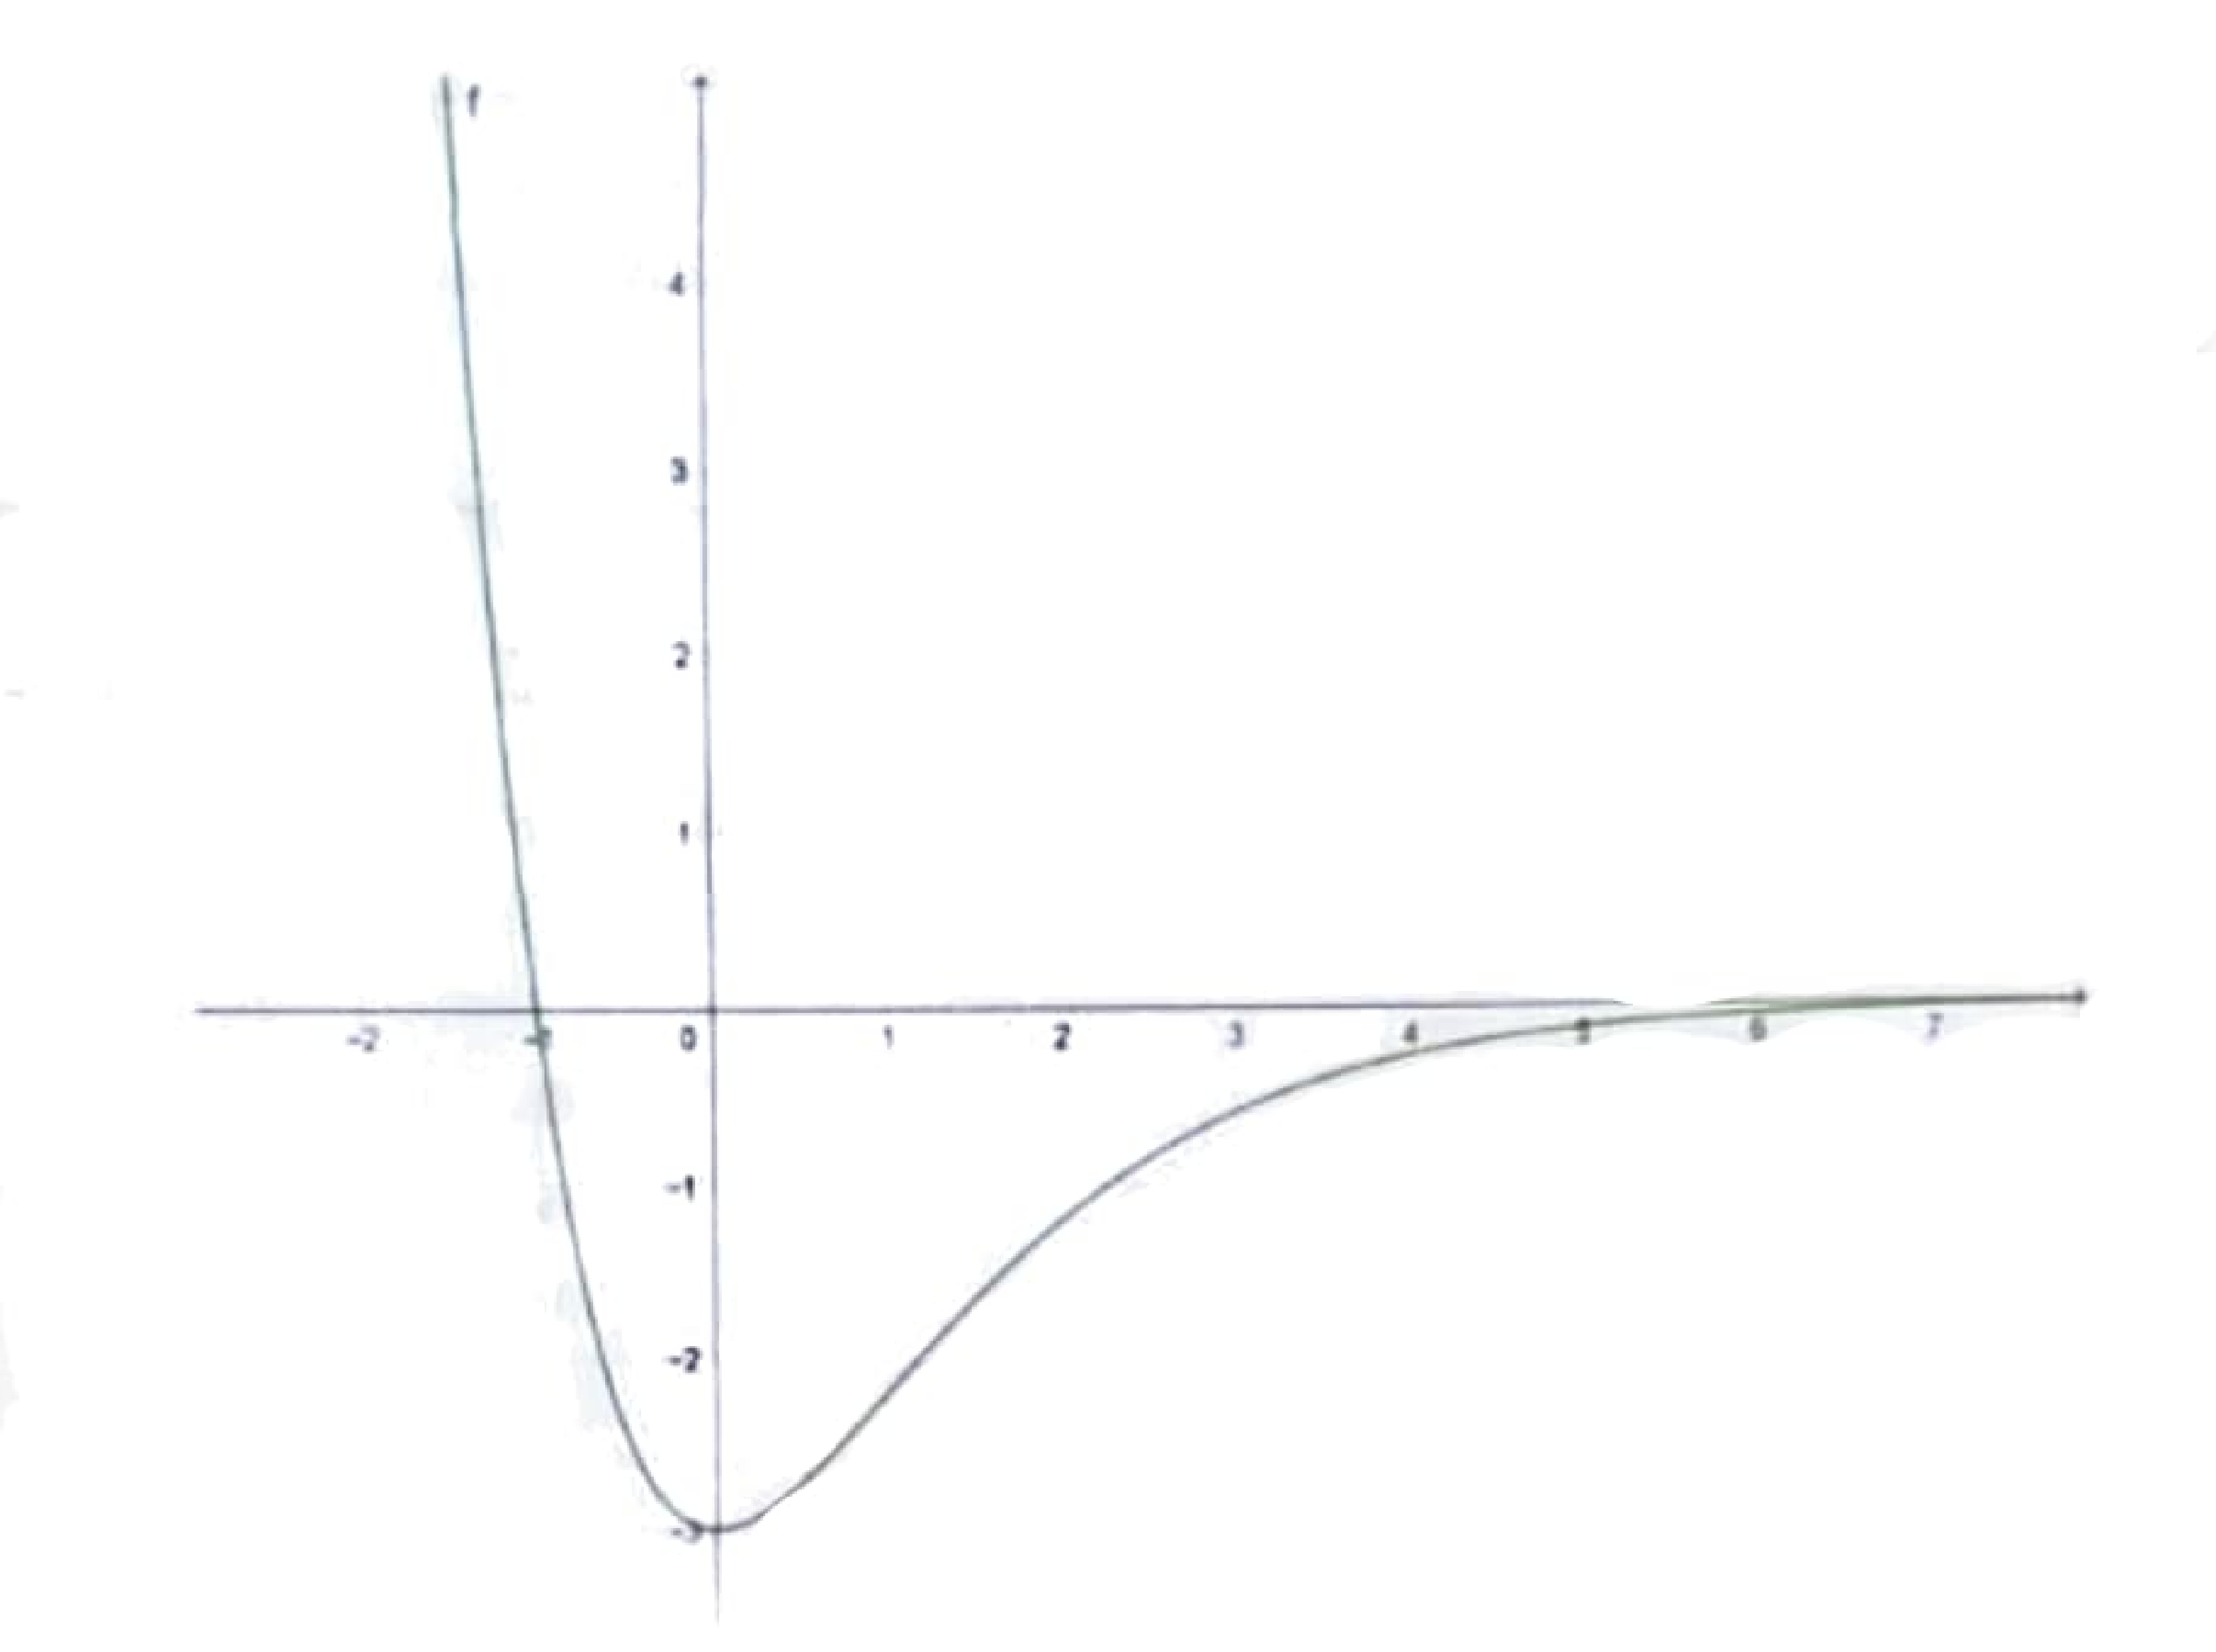
\includegraphics[width=70mm]{g3.jpg}
\end{figure}


  \begin{enumerate}[label={\alph*)}]
    \item Zeigen Sie, dass $F$ mit $F: x \rightarrow 3e^{-x}(x+2)$ die Stammfunktion von $f(x)$ ist.
    \item Bestimmen Sie die Flache zwischen dem Graphen und der x-Achse im Intervall [-1:0]
    \item Welche Informationen kann man über den Verlauf der Funktion $f'$ gewinnen?
  \end{enumerate}

\item Gegeben ist die Funktion $g:x \rightarrow -4\ln{(x+3)}$ mit der Definitionsmenge $D_g$.

  \begin{enumerate}[label={\alph*)}]
    \item Beschreiben Sie, wie $G_g$ aus dem Graphen der Funktion $x \rightarrow \ln x$ hervorgeht.
    \item Bestimmen Sie die Nullstelle, Definitions- und Wertemenge der Funktion $g$
    \item Bestimmen Sie die Gleichung der Tangente im Punkt $(-2 | f(-2))$.
  \end{enumerate}
\end{enumerate}

\newpage

\underline{\textbf{Geometrie}}

\begin{enumerate}
  \item In einem Koordinatensystem sind die Punkte $A(3|-1|1), B(8|0|2), C(5|0|1), D(1|-1|0)$ sowie die Gerade $g:\vec{x} = \begin{pmatrix} 4 \\ -5 \\ -2 \end{pmatrix} + \alpha \begin{pmatrix} 2 \\ -2 \\ 0 \end{pmatrix}$ gegeben.

  \begin{enumerate}[label={\alph*)}]
    \item Bestimmen Sie die Gleichung der Ebene $E$ die durch die Punkte $A, B$ und $C$ aufgespannt wird in Parameter- und Koordinatenform.\\
      {[Kontrolle:$-x_1+2x_2+3x_3+2=0$]}

  \item Untersuchen Sie die Lagebeziehung der Geraden $g$ und der Ebene $E$. Beschreiben Sie gegebenenfalls wie man den Schnittpunkt und den Schnittwinkel bestimmen kann.

  \item Welche besondere Lage hat im Koordinatensystem die Gerade $g$?

  \item Bestimmen Sie den Abstand des Punktes $D$ von der Ebene $E$.
  \end{enumerate}
\end{enumerate}

\end{document}

